\documentclass[final,twocolumn]{fhnwreport}
%%---Main Packages-----------------------------------------------------------------------
\usepackage[english, ngerman]{babel}	%Mul­tilin­gual sup­port for LaTeX
\usepackage[T1]{fontenc}				      %Stan­dard pack­age for se­lect­ing font en­cod­ings
\usepackage[utf8]{inputenc}				  %Ac­cept dif­fer­ent in­put en­cod­ings
\usepackage{lmodern}                 %The newer Font-Set
\usepackage{textcomp}					      %LaTeX sup­port for the Text Com­pan­ion fonts
\usepackage{graphicx} 					      %En­hanced sup­port for graph­ics
\usepackage{float}						        %Im­proved in­ter­face for float­ing ob­jects
%\usepackage{ifdraft}                %Let you check if the doc is in draft mode

%%---Useful Packages---------------------------------------------------------------------
\usepackage[pdftex,dvipsnames]{xcolor}  %Driver-in­de­pen­dent color ex­ten­sions for LaTeX
\usepackage{csquotes}                   %Simpler quoting with \enquote{}
\usepackage{siunitx} 					     %A com­pre­hen­sive (SI) units pack­age
\usepackage{listings}					     %Type­set source code list­ings us­ing LaTeX
\usepackage[bottom]{footmisc}			  %A range of foot­note op­tions
\usepackage{footnote}					     %Im­prove on LaTeX's foot­note han­dling
\usepackage{verbatim}					     %Reim­ple­men­ta­tion of and ex­ten­sions to LaTeX ver­ba­tim
\usepackage[textsize=footnotesize]{todonotes} %Mark­ing things to do in a LaTeX doc­u­ment
\usepackage{lipsum}              % Gives you access to blindtext

%%---Tikz Packages-----------------------------------------------------------------------
%\usepackage{standalone}
%\usepackage{tikz}
%\usepackage{circuitikz}
%\usetikzlibrary{arrows}
%\usetikzlibrary{calc}
%\usetikzlibrary{intersections}

%%---Math Packages-----------------------------------------------------------------------
\usepackage{amsmath}					    %AMS math­e­mat­i­cal fa­cil­i­ties for LaTeX
%\usepackage{amssymb}					  %Type­set­ting symbols (AMS style)
%\usepackage{array}						  %Ex­tend­ing the ar­ray and tab­u­lar en­vi­ron­ments
%\usepackage{amsthm}					    %Type­set­ting the­o­rems (AMS style)

%%---Table Packages----------------------------------------------------------------------
\usepackage{tabularx}					  %Tab­u­lars with ad­justable-width columns
%\usepackage{longtable}
\usepackage{multirow}					  %Create tab­u­lar cells span­ning mul­ti­ple rows
\usepackage{multicol}					  %In­ter­mix sin­gle and mul­ti­ple columns

%%---PDF / Figure Packages---------------------------------------------------------------
\usepackage{pdfpages}					  %In­clude PDF doc­u­ments in LaTeX
\usepackage{pdflscape}					  %Make land­scape pages dis­play as land­scape
%\usepackage{subfig}					    %Fig­ures di­vided into sub­fig­ures

%%---Other Packages----------------------------------------------------------------------
%\usepackage{xargs}              %De­fine com­mands with many op­tional ar­gu­ments


%%---Main Settings-----------------------------------------------------------------------
\graphicspath{{./graphics/}}			%Defines the graphicspath
%\geometry{twoside=false}				%twoside=false disables the "bookstyle"
\setlength{\marginparwidth}{2cm}
\overfullrule=0pt						    %Creates a black rule if text goes over the margins => debugging

%%---User Definitions--------------------------------------------------------------------
%%Tabel-Definitions: (requires \usepackage{tabularx})
\newcolumntype{L}[1]{>{\raggedright\arraybackslash}p{#1}}    %column-width and alignment
\newcolumntype{C}[1]{>{\centering\arraybackslash}p{#1}}
\newcolumntype{R}[1]{>{\raggedleft\arraybackslash}p{#1}}					

\usepackage{amsfonts,amssymb}

\usepackage[
  activate={true,nocompatibility}, % Aktiviert Protrusion und Expansion
  final,                          % Sorgt dafür, dass microtype auch im Draft-Modus aktiv ist
  tracking=true,                  % Aktiviert das Letterspacing (Tracking)
  kerning=true,                   % Aktiviert zusätzliches Kerning
  spacing=true,                   % Optimiert die Abstände zwischen Wörtern
  factor=1000,                    % Erhöht den Protrusion-Effekt leicht (Standard: 1000)
  stretch=20,                     % Begrenzt die Schriftausdehnung (Standard: 20)
  shrink=20                       % Begrenzt die Schriftschrumpfung (Standard: 20)
]{microtype}

\newcommand{\logofilename}{FHNW_HSI_DE}

\usepackage[style=ieee,urldate=comp,backend=biber]{biblatex}
\addbibresource{literature/Citations.bib}

\title{Quaternion-Valued Neural Networks and Predictive Coding}
\author{Lukas Breiter}
\date{Windisch, Mai 2026}

\begin{document}

\pagenumbering{roman}

\selectlanguage{ngerman}
\onecolumn
\thispagestyle{empty}
\begin{center}
\includegraphics[height=12mm]{\logofilename}\\[2.0cm]
{\Large\bfseries FHNW Hochschule für Technik und Umwelt}\\[0.6cm]
{\LARGE\bfseries Quaternion-Valued Neural Networks and Predictive Coding}\\[0.8cm]
{\large Projektbericht im Modul OML}\\[1.2cm]
\begin{tabular}{@{}ll@{}}
Student: & Lukas Breiter\\
Fachexperte: & Michael Graber\\
Datum: & Windisch, Mai 2026\\
\end{tabular}
\end{center}

\vfill
\begin{center}
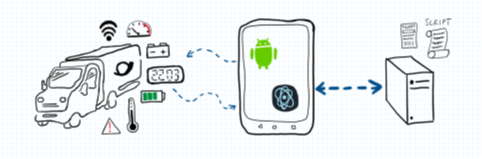
\includegraphics[width=0.9\textwidth]{graphics/titleimage.png}
\end{center}

\section*{Abstract}
Dieser Bericht untersucht die Optimierung quaternionwertiger neuronaler Netzwerke auf vier nichtlinearen vierdimensionalen Regressionsbenchmarks: Ackley, Griewank, Rastrigin und Schwefel. Der Fokus liegt nicht auf einer neuen Modellarchitektur allein, sondern auf der Frage, welche Optimierungsdynamik entsteht, wenn klassische Quaternion-Backpropagation mit Predictive Coding verglichen wird. Als Baselines werden CMLP und GHR reproduziert; danach werden ein reellwertiges Predictive Coding Network (PCN) und eine split-quaternion Variante (CPCN) untersucht. CMLP bleibt auf Ackley, Griewank und Rastrigin die stärkste Baseline, waehrend GHR auf Schwefel leicht besser abschneidet. Das reellwertige PCN reduziert zwar teilweise interne Rekonstruktionsfehler, liefert in der freien Test-Inferenz aber keine brauchbare Funktionsapproximation. CPCN ist numerisch stabiler und erreicht kleinere Fehler als das reellwertige PCN, erklaert auf der Testmenge jedoch noch fast keine Varianz. Das Resultat ist damit folgendes: In $\mathbb{H}$ bzw. in der $\mathbb{R}^4$-Darstellung sind Lernrate, Batchgroesse, Produktreihenfolge, latente Inferenz und Testmodus stark gekoppelt. Predictive Coding ist für QVNNs implementierbar, führt aber in der aktuellen Konfiguration nicht automatisch zu konkurrenzfähiger Generalisierun und benötigt warscheinlich eine grosse Hyperparametersuche.
\vspace{2ex}

\clearpage

\twocolumn
\pagenumbering{arabic}
\setcounter{page}{1}
\section{Einleitung}

Quaternionwertige neuronale Netzwerke (QVNNs) verarbeiten Eingaben, Gewichte und Aktivierungen nicht als einzelne reelle Zahlen, sondern als Quaternionen. Ein Quaternion
\[
q = q_0 + q_1\mathbf{i} + q_2\mathbf{j} + q_3\mathbf{k}
\]
besteht aus vier gekoppelten reellen Komponenten. Das ist fuer Daten interessant, bei denen mehrere Komponenten zusammengehoeren, etwa bei Rotationen, Farbinformationen oder mehrdimensionalen Signalen. In solchen Faellen koennen QVNNs kompaktere Modelle und teilweise bessere Generalisierung liefern als vergleichbare reellwertige Netzwerke \cite{bill2023comparison,article}. Gleichzeitig ist die Optimierung schwieriger, weil das Hamilton-Produkt nicht kommutativ ist. Die Reihenfolge von Faktoren ist also relevant; Standard-Backpropagation laesst sich nicht ohne Anpassung uebertragen.

Aus Sicht des Moduls OML ist genau diese Optimierungsfrage zentral. Bill, Cox und Champagne vergleichen mehrere Quaternion-Backpropagation-Verfahren und zeigen, dass bereits kleine Unterschiede in Lernregel, Produktreihenfolge und Hyperparametern deutliche Auswirkungen auf Genauigkeit und Laufzeit haben koennen \cite{bill2023comparison}. In ihrer Studie erreicht der Clifford Multilayer Perceptron (CMLP) auf mehreren Regressionsbenchmarks die staerkste Gesamtleistung. Dieses Projekt nimmt CMLP deshalb als Optimierungsbaseline und fragt, ob Predictive Coding eine brauchbare Alternative oder Erweiterung fuer QVNNs sein kann.

Predictive Coding Networks (PCNs) verwenden keine reine Feedforward-Aktivierungskette. Stattdessen versucht jede Schicht, die Aktivitaet der darunterliegenden Schicht vorherzusagen. Bei festen Gewichten werden zuerst latente Zustaende iterativ inferiert; erst danach werden die Gewichte anhand lokaler Vorhersagefehler aktualisiert \cite{stenlund2025pcn}. Ein PCN ist deshalb nicht nur ein anderer Optimierer fuer ein MLP, sondern eine eigene Lernarchitektur mit zwei Zeitskalen: schnelle Inferenz und langsameres Gewichtslernen. Dadurch entstehen zusaetzliche Optimierungsentscheidungen, insbesondere Inferenzschrittweite, Anzahl Inferenzschritte, latente Initialisierung, Lernrate und Batchgroesse.

Die Fragestellung des Projekts lautet daher:

\begin{quote}
Laesst sich ein quaternionwertiges neuronales Netzwerk mit Predictive Coding auf Standardaufgaben zur Approximation nichtlinearer Funktionen stabil optimieren, und wie verhaelt sich diese Optimierung im Vergleich zu starken Quaternion-Backpropagation-Baselines?
\end{quote}

Der Bericht konzentriert sich auf diese Optimierungsfrage. Die theoretischen Grundlagen werden nur so weit eingefuehrt, wie sie fuer Methodik und Interpretation notwendig sind. Der Schwerpunkt liegt auf den implementierten Modellen, den Hyperparametern, den Resultaten und den beobachteten Trainingsdynamiken.

\section{Grundlagen}

\subsection{Quaternionen und QVNNs}

Die Quaternionen $\mathbb{H}$ erweitern die komplexen Zahlen um drei imaginäre Einheiten $\mathbf{i},\mathbf{j},\mathbf{k}$. Für diese gelten
\[
\begin{aligned}
\mathbf{i}^2&=\mathbf{j}^2=\mathbf{k}^2=-1,\\
\mathbf{i}\mathbf{j}&=\mathbf{k},\quad
\mathbf{j}\mathbf{k}=\mathbf{i},\quad
\mathbf{k}\mathbf{i}=\mathbf{j}.
\end{aligned}
\]
Vertauscht man die Reihenfolge, ändert sich das Vorzeichen. Deshalb ist das Hamilton-Produkt im Allgemeinen nicht kommutativ. In einem QVNN werden die linearen Operationen eines MLP durch quaternionwertige Operationen ersetzt. Eine Schicht kann vereinfacht als
\[
s_j^{(l)} = \phi\left(\sum_i w_{ji}^{(l)} \otimes s_i^{(l-1)} + b_j^{(l)}\right)
\]
geschrieben werden. Dabei sind $s$, $w$ und $b$ Quaternionen, $\otimes$ ist das Hamilton-Produkt und $\phi$ ist meist eine split-Aktivierung: Eine reellwertige Aktivierungsfunktion wird komponentenweise auf $q_0,q_1,q_2,q_3$ angewendet.

Der Vorteil dieser Darstellung ist die kompakte Kopplung von vier Komponenten. Der Nachteil liegt in der Optimierung. Ein Quaternion kann zwar als Vektor in $\mathbb{R}^4$ gespeichert werden, die vier Komponenten sind durch das Hamilton-Produkt aber nicht unabhängig. Konjugationen und Produktreihenfolgen bestimmen die Richtung des Updates. Dadurch können Gradientenkomponenten, die in einem reellen Netzwerk unproblematisch gemittelt werden, in $\mathbb{H}$ gegeneinander arbeiten. Die Baselines in diesem Projekt sind deshalb nicht reellwertige MLPs, sondern quaternionwertige Lernregeln aus der Literatur.

\subsection{CMLP und GHR als Baselines}

Der CMLP-Ansatz stammt aus der Clifford-Algebra-Perspektive und verwendet split Aktivierungen sowie eine komponentenweise Pseudoableitung. Für Quaternionen ergibt sich eine praktische Lernregel, bei der Fehlerterme mit konjugierten Aktivierungen bzw. Gewichten kombiniert werden \cite{buchholz2008cmlp,bill2023comparison}. Weil CMLP in der Vergleichsstudie von Bill et al. auf mehreren Regressionsaufgaben am besten abschneidet, dient CMLP hier als Hauptreferenz \cite{bill2023comparison}.

GHR steht für Generalized Hamilton-Real Calculus. Dieser Kalkül formuliert Ableitungen in $\mathbb{H}$ formaler und verwendet Ableitungen bezüglich $q$ und $q^*$ \cite{xu2015enabling}. GHR ist mathematisch reichhaltiger, aber in der Implementierung aufwendiger.

\subsection{Predictive Coding Networks}

Ein PCN besitzt latente Variablen $x^{(1)},\dots,x^{(L)}$ und eine beobachtete Eingabe $x^{(0)}$. Jede Schicht $l+1$ sagt die darunterliegende Schicht $l$ voraus:
\[
\begin{aligned}
a^{(l)} &= W^{(l)}x^{(l+1)},\\
\hat{x}^{(l)} &= f(a^{(l)}),\\
\varepsilon^{(l)} &= x^{(l)}-\hat{x}^{(l)}.
\end{aligned}
\]
Die Energie des Netzwerks ist die Summe der lokalen Vorhersagefehler:
\[
\mathcal{E}=\frac{1}{2}\sum_{l=0}^{L-1}\left\|\varepsilon^{(l)}\right\|^2.
\]
Beim Training werden zuerst die latenten Zustände durch mehrere Inferenzschritte angepasst. Danach werden die Gewichte aktualisiert. Diese Trennung ist zentral: Ein PCN kann intern eine niedrige Free Energy erreichen, ohne dass die freie Test-Inferenz bereits eine gute Vorhersage liefert. Genau dieser Unterschied zwischen interner Fehlerreduktion und Generalisierung ist in den Experimenten sichtbar.

Für supervised Learning wird ein Output-Fehler ergänzt. Während des Trainings kann der Zielwert in die Inferenz einbezogen werden. Bei der Auswertung muss die Vorhersage dagegen ohne bekannten Zielwert durch freie Inferenz entstehen \cite{stenlund2025pcn,whittington2017approximation,millidge2022predictive}. Optimierungstechnisch unterscheidet sich ein PCN damit deutlich von einem klassischen NN: Neben der Gewichtsanpassung muss auch das Inferenzverfahren stabil sein. Ein scheinbar sinkender Trainingsfehler ist deshalb nur dann aussagekräftig, wenn die gleiche Konfiguration auch ohne geklemmtes Ziel sinnvolle Testvorhersagen erzeugt.

\section{Architektur}

\lipsum[27]
\section{Resutate}

\lipsum[27]
\section{Diskussion und Ausblick}

\lipsum[28]



\
{\sloppypar
\printbibliography[heading=bibintoc, title=Quellenverzeichnis]
}


\end{document}